\section{Overview}
The system simulates a population of individuals, termed ``blobs", whose sole purpose is continued existence. This is achieved thorugh continuous feeding, followed eventually by reproduction. The latter is done asexually; when each individual reaches a sufficient energy threshold encoded in its internal state. Energy can be gained by eating food pellets scattered randomly around the world. The blobs eat food by colliding with it, and find it by performing a random walk, in this case, a simplified version of a L\'evy walk\cite{matthaus2009coli}.

The system is designed with interactivity in mind, allowing the user to alter various parameters of the environment, while observing how the population evolves in order to adapt to the change. A user could interact more directly with the simulation by adding blobs or placing food. A sudden influx in either will generate a period of instability in the population which eventually reverts back to a stable state. Information about the population is presented via a graph, showing total number and average characteristics of the individuals. More specific information about a blob in particular is displayed via a pop-up message, should a creature be clicked on.

\subsection{Definitions}
In order to provide a better understanding, some terms are defined below:

\begin{itemize}
	\item Blob --- A single creature in the simulation;
	\item Food --- A nutritional pellet, providing Energy to whomever eats it;
	\item Population --- The set containing all blobs: at a certain time;
	\item Energy --- A blob's measure of how healthy it is. This triggers death at low values;
	\item Patience --- The time measured in number of ticks until a blob leaves a certain area.
	\item Reproduction --- The act of division of a blob when an energy threshold is reached;
	\item Genome --- A simulated DNA string in which the parameters of a blob are encoded.
	\item Mutation --- The act of a single bit in the genome becoming inverted at random.
\end{itemize}

\subsection{Goals and Considerations}

As the main purpose of the system is that of a teaching aid, it was designed with the primary goal of interactivity in mind. This resulted in a need for a visualisation as an effective way of conveying information. A visual component would present the state of the system, and at the same time, it would allow the user to directly interact with the simulation in real-time. A further goal was portability; due to the variety of platforms available, allowing the simulation to run on as many as possible became of paramount importance. As such, the final version of the system is built using the Unity Game Engine\cite{unitywebsite}.

\section{Design Process}
Before any implementation work was carried out, the system specifications were laid out. Based on the pre-established requirements (Chapter~\ref{requirements}), a plan of the system was drafted. An early draft can be seen in Figure~\ref{fig:initial2}. This plan was further refined into the existing architecture, currently containing two logical components: the visualisation, and the simulation logic. The characteristics of an individual blob were also discussed, together with a set of basic behaviours, as seen in Figure~\ref{fig:initial3}.

\begin{figure}[!th]
	\centering
	\begin{minipage}[b]{0.40\textwidth}
		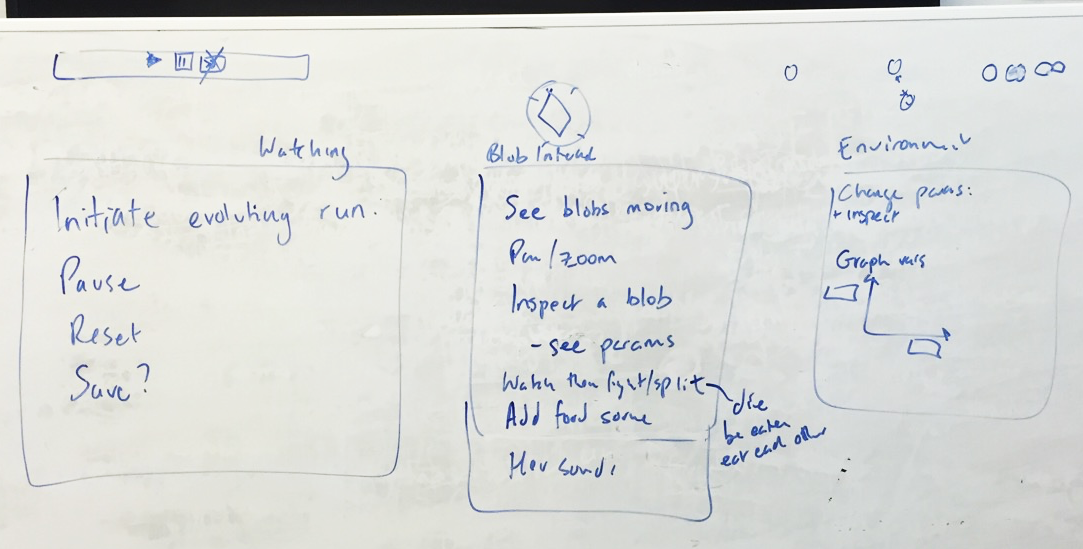
\includegraphics[scale=0.34]{images/initial2}
		\caption{\label{fig:initial2}The base functions of the system, split into logical components}
	\end{minipage}
	\hfill
	\begin{minipage}[b]{0.45\textwidth}
		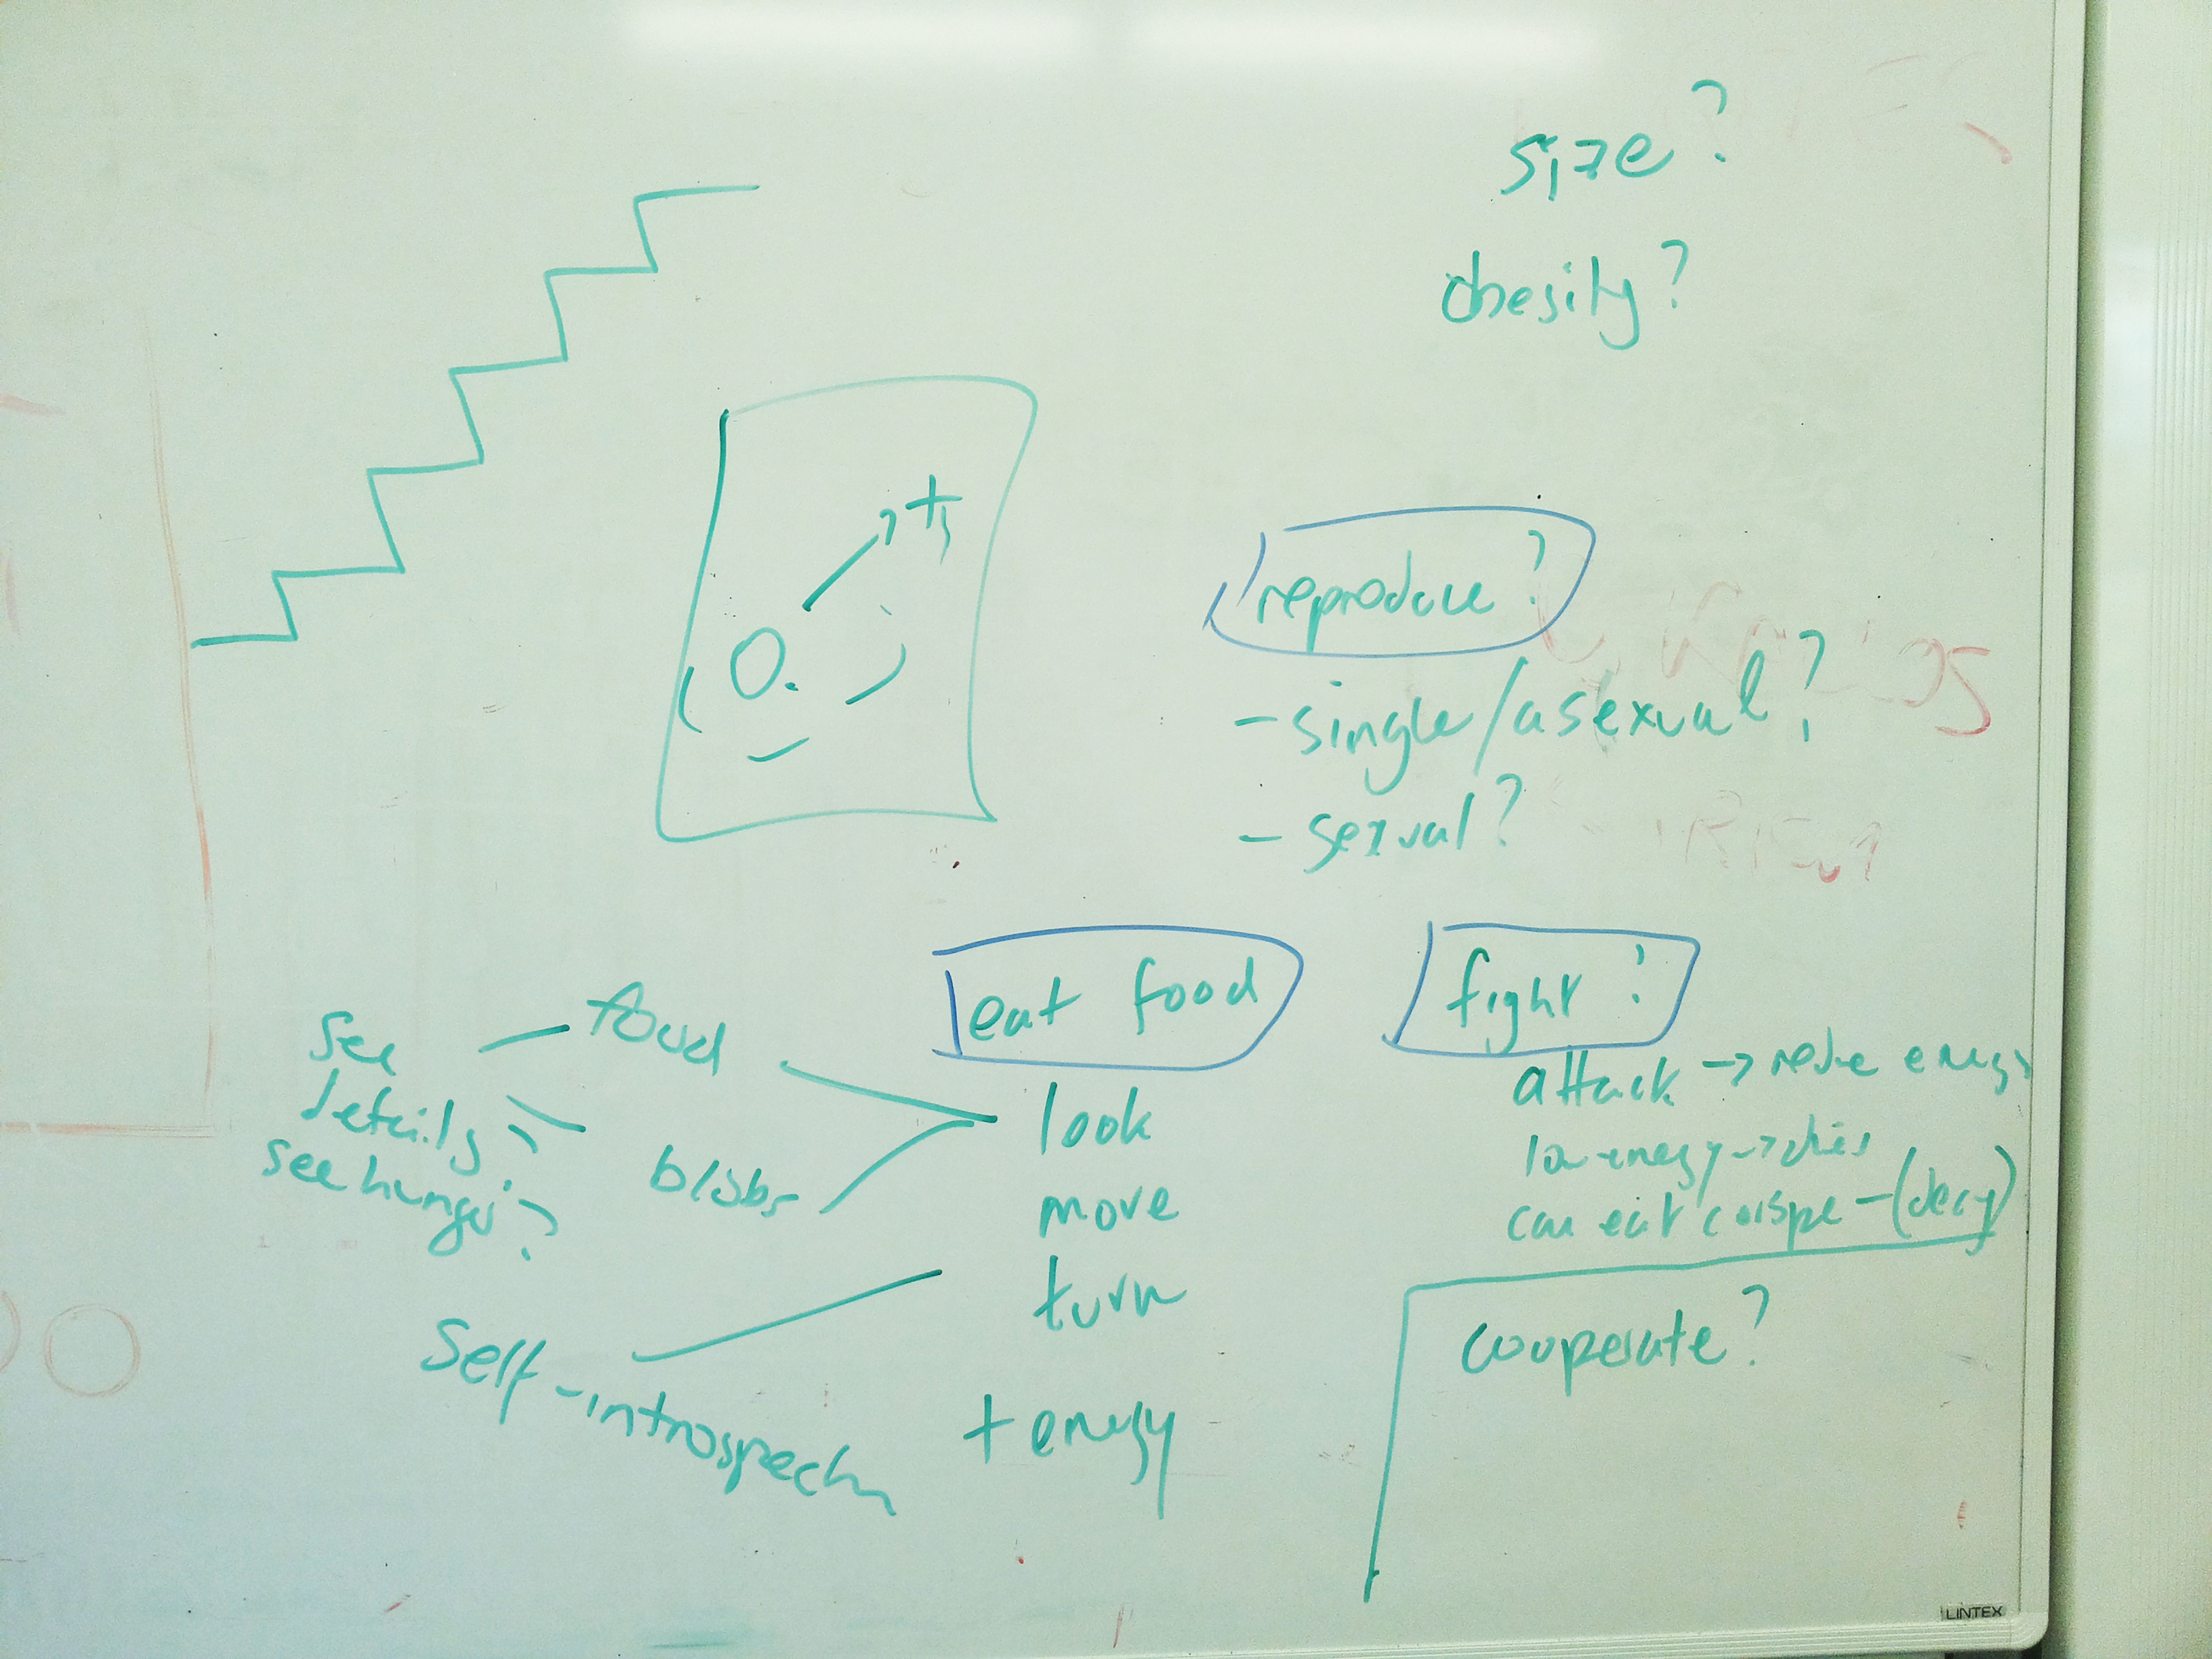
\includegraphics[scale=0.07]{images/initial3}
		\caption{\label{fig:initial3}Initial blob characteristics and behaviour}
	\end{minipage}
\end{figure}

\subsection{Simulation Type}
The system is an agent-based model (ABM), as it focuses on simulating individual blobs. ABMs are often used in biology as the mapping from the simulated entities to their real-world equivalents is straightforward. The paper ``Agent-based models in translational systems biology"\cite{an2009agent} highlights the advantages of ABMs for biological systems. Noteworthy are the characteristic representation of space and strongly-enforced rules, as the origins of ABMs are cellular automatons, and the stochastic nature of the individuals inside the simulation. Despite the simplicity of the simulation, the emergent property is still verified, as complex population dynamics can be observed from uncomplicated individuals.

Similar to most agent-based models, the system is discrete event simulation\cite{robinson2014simulation}. The simulation advances only on update ticks which can happen with varying frequency, between 1 and 60 ticks per second. The speed of the ticks is controlled by the user. From a spatial perspective, however, the system is continuous, as a blob can occupy any position on the plane, unrestricted by any imposed grid; this was done in order to provide a greater freedom of movement.

\subsection{Framework selection}
During the initial stages of the projects, several development platforms and frameworks were explored. Among the initial choices were Windows Forms Application, and a more general DirectX based, .NET implementation. These, however, proved inadequate, either due to performance issues in the former, or portability issues which both suffered from. While this line of implementation was stopped, elements of the interface design were kept.

A later implementation was attempted in Mono\cite{monoproject}, an open-source .NET framework built with platform portability in mind. This solved the concern of cross-platform, but did not provide a viable solution for the visualisation, as the existing portable GUI tool-kits for Mono proved difficult to work with. As such, Mono was dropped as an implementation choice.

The final incarnation of the project, is implemented in the Unity Game Engine. Due to its intended nature as a game engine, the performance issues previously encountered with other tool-kits were not present. Unlike Mono, Unity also offered a built-in way of designing the user interface. In order to target a larger audience, the project could be compiled to run on any of the three major platforms (Windows, MacOS, Linux), as well as mobile platforms, and web browsers, via the Unity Web Player. Together with the Asset Store allowing the import of plug-ins, Unity became the framework of choice. A screenshot of the final project open in the Unity Editor can be seen in Figure~\ref{fig:unityfinal}.

A comparison of the previously presented frameworks can be found in Table~\ref{table:frameworkscomp}.

\begin{table}[!th]
	\centering
	\begin{tabular}{|c|c|c|c|c|c|c|}
		\hline
						& Performance & Portability & Ease-of-use & Language & Community support \\ \hline
		Windows Forms   & $\times$      & $\times$      & $\checkmark$  & C++, C\# & $\times$     \\ \hline
		.NET            & $\checkmark$  & $\times$      & $\checkmark$  & C++, C\# & $\checkmark$ \\ \hline
		Mono            & $\checkmark$  & $\checkmark$  & $\times$      & C++, C\# & $\checkmark$ \\ \hline
		Unity           & $\checkmark$  & $\checkmark$  & $\checkmark$  & C\#      & $\checkmark$ \\ \hline
	\end{tabular}
	\caption{\label{table:frameworkscomp}Comparison between explored frameworks}
\end{table}

\begin{figure}[!th]
	\centering
	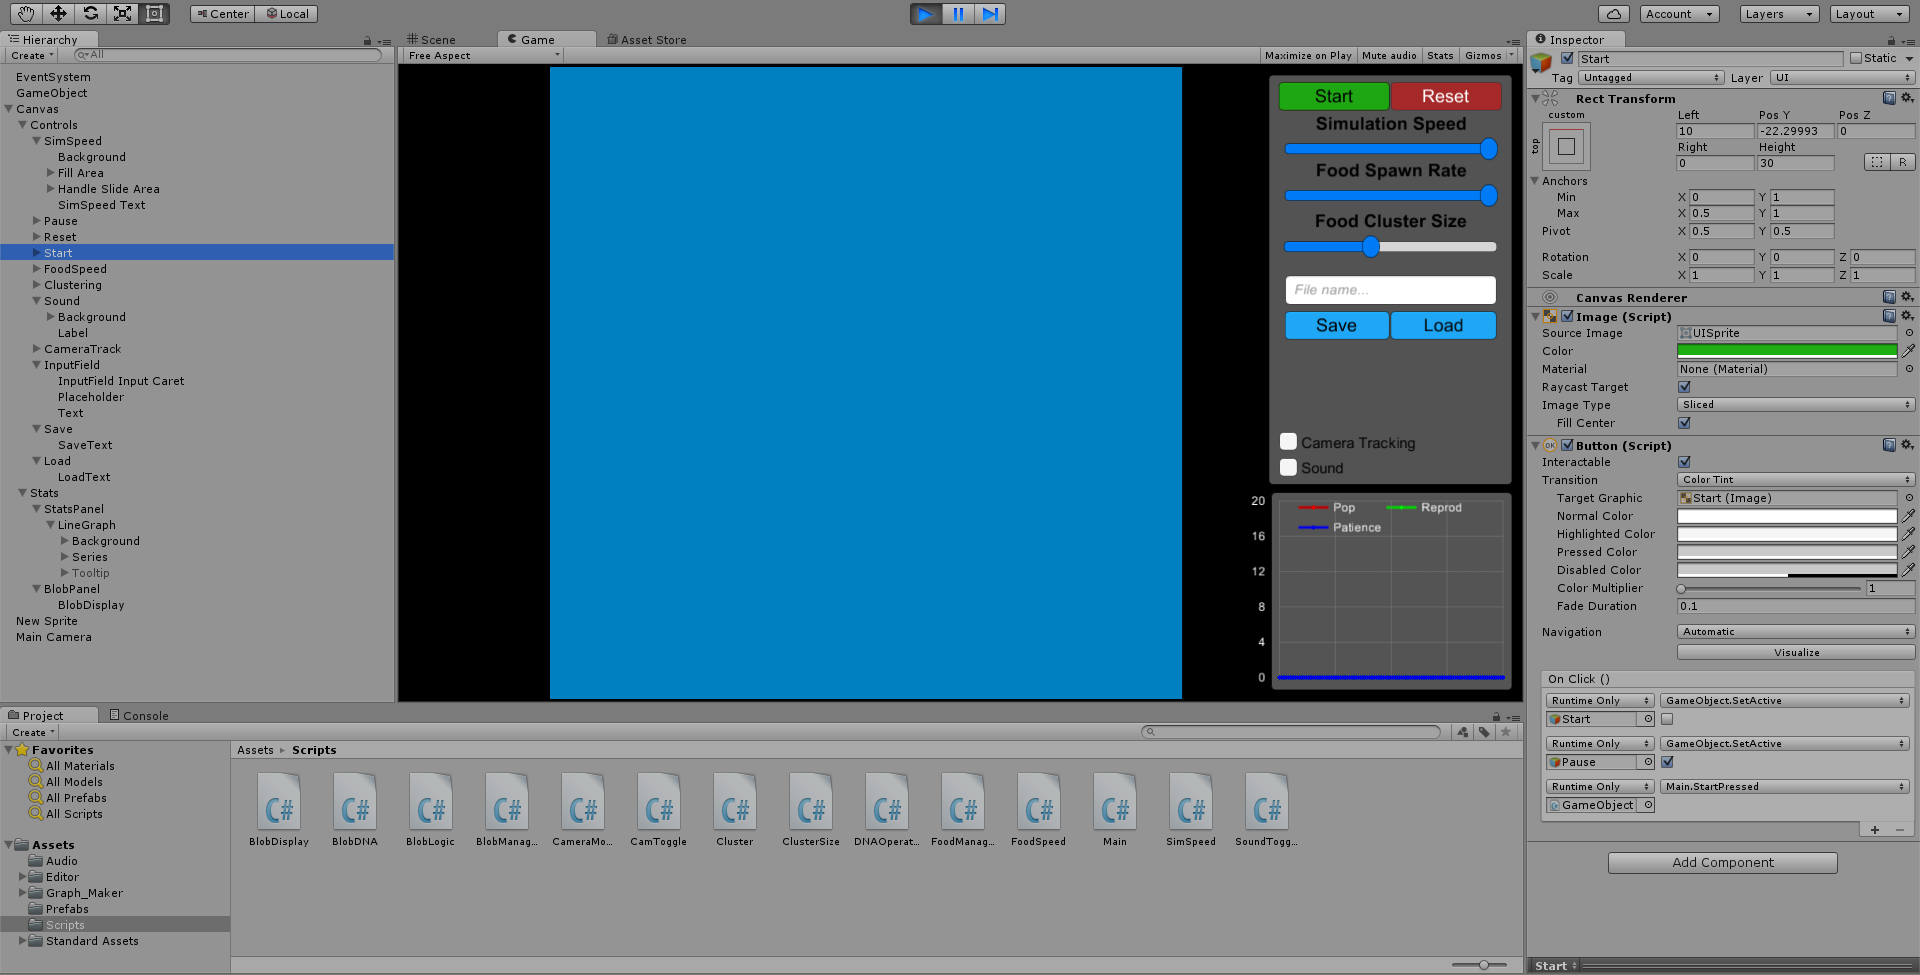
\includegraphics[scale=0.35]{images/unityfinal}
	\caption{\label{fig:unityfinal}The Unity Editor running the system}
\end{figure}

\section{Architecture}

The underlying architectural pattern of the system is the Model-View-Controller (MVC) design pattern. Initially introduced in the late 1970s, MVC was described by its creator in ``The original MVC reports"\cite{reenskaug1979original} as a solution for users handling complex data sets. A diagram of how MVC is applied to the system is presented in Figure~\ref{fig:mvc}. The arrows represent channels of interaction: whether direct manipulation by an user through the user interface, data paths in the system, or visual feedback on the screen. The user interacts with the controller pictured in yellow, which modifies the data in the model, depicted in blue for blob data and green for food-related data. This in turn is reflected in the view, coloured in purple, presented back to the user. MVC is used in order to provide separation between the user interface, the visualization, and the simulation logic. Such separation allows changes to either of the three components with relative ease and minimises the impact on the others. An informal diagram detailing the interaction between the classes directly involved in the simulation can be seen in Figure~\ref{fig:mmodel}.

\begin{figure}[!th]
	\centering
	\includegraphics[scale=0.6]{images/mvc}
	\caption{\label{fig:mvc}The design of the system as an MVC}
\end{figure}

\begin{figure}[!th]
	\centering
	\includegraphics[scale=0.5]{images/mmodel}
	\caption{\label{fig:mmodel}Informal class diagram}
\end{figure}

\section{Interface}

The design of the interface was an iterative process, starting from whiteboard and paper prototypes, continuing with partial, non-functional implementations, and arriving at a usable interface, built in Unity. The user evaluation proved key, as some of the feedback received (Section~\ref{usereval}) was used in the redesigns. This incremental process complemented the Agile development method employed. A detailed view on how Agile was used in order to build the system can be found in Section~\ref{projmgmt}. 

\subsection{Interface iterations}
While the initial interface sketches were crude, they quickly converged towards a more stable, intermediate design. Some of the initial prototypes can be seen in Figure~\ref{fig:test1}, as well as Figure~\ref{fig:test2}.

\begin{figure}[!th]
	\centering
	\begin{minipage}[b]{0.45\textwidth}
		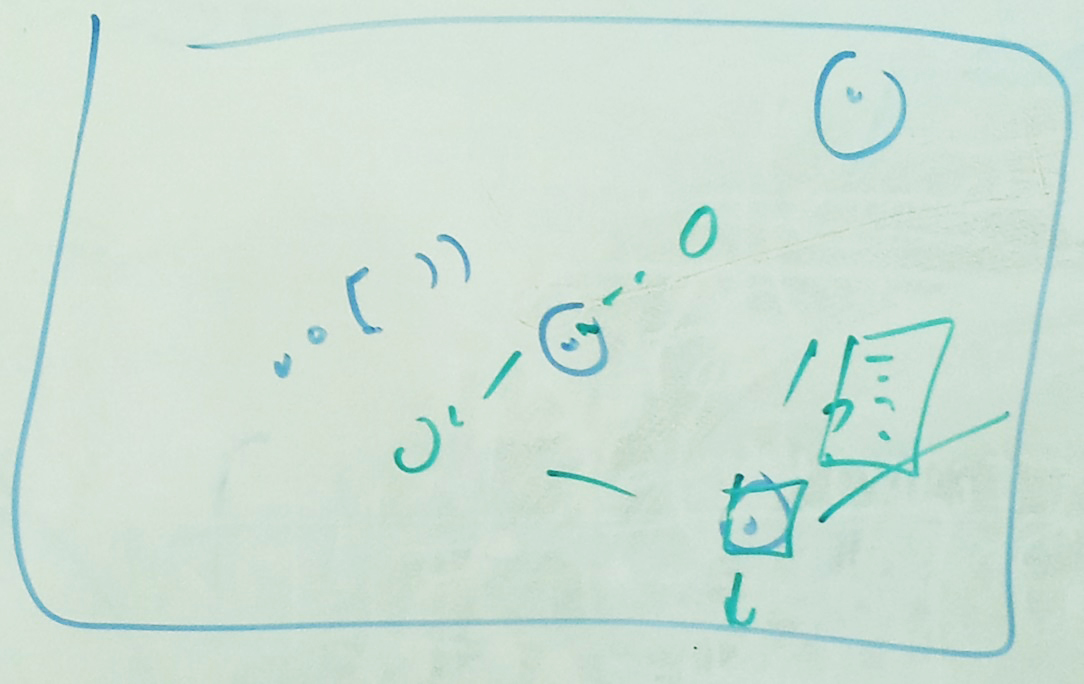
\includegraphics[scale=0.24]{images/testinterface2}
		\caption{\label{fig:test1}The base functions of the system, split into logical components}
	\end{minipage}
	\hfill
	\begin{minipage}[b]{0.45\textwidth}
		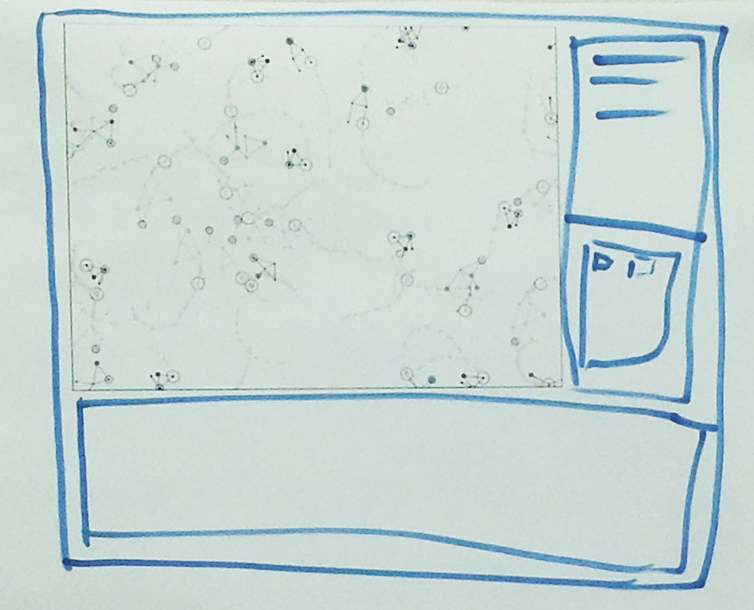
\includegraphics[scale=0.27]{images/testinterface}
		\caption{\label{fig:test2}Initial blob characteristics and behaviour}
	\end{minipage}
\end{figure}

Following the initial designs, a computer-assisted prototype was created. Even though this was non-functional, it served as a baseline for any subsequent iterations. A mock implementation can be seen in Figure~\ref{fig:uitest}. This includes the environmental controls via the sliders, as well displays containing information about a selected blob and the population in general.

\begin{figure}[!th]
	\centering
	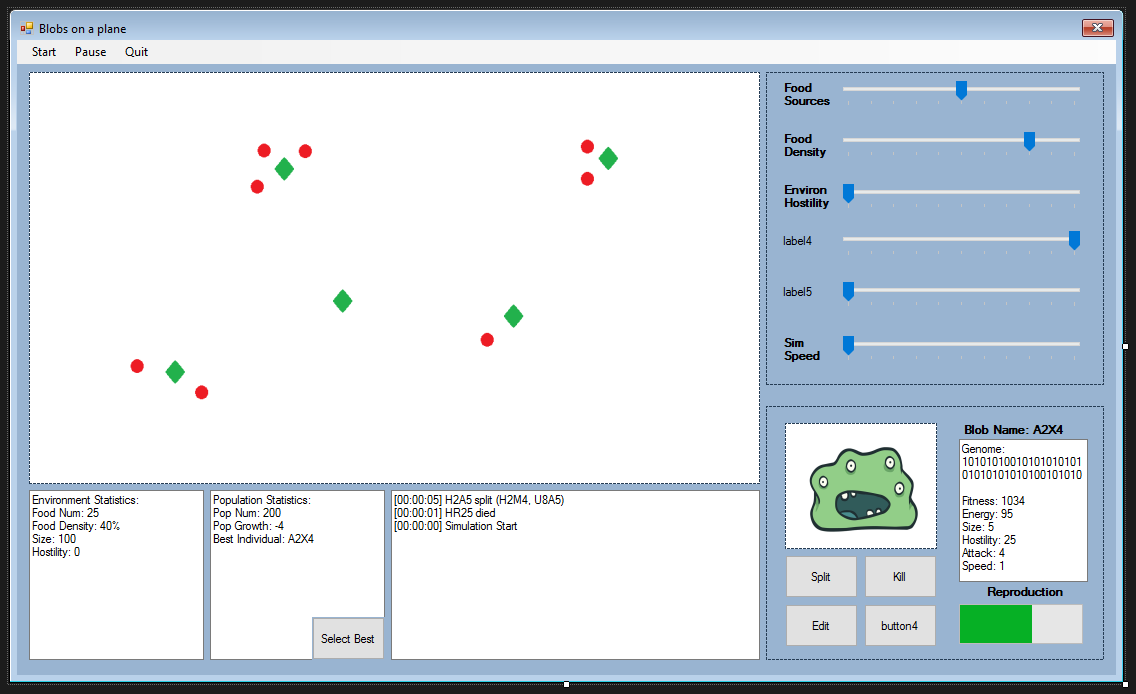
\includegraphics[scale=0.45]{images/uitest}
	\caption{\label{fig:uitest}User Interface and Visualisation build in Windows Forms Application}
\end{figure}

After the transition to Unity, the interface was remade using the build-in Unity UI tools. Information about the population is also displayed via a rudimentary histogram in the top-left corner of the screen. An intermediary design can be seen in Figure~\ref{fig:unitypart}. 

\begin{figure}[!th]
	\centering
	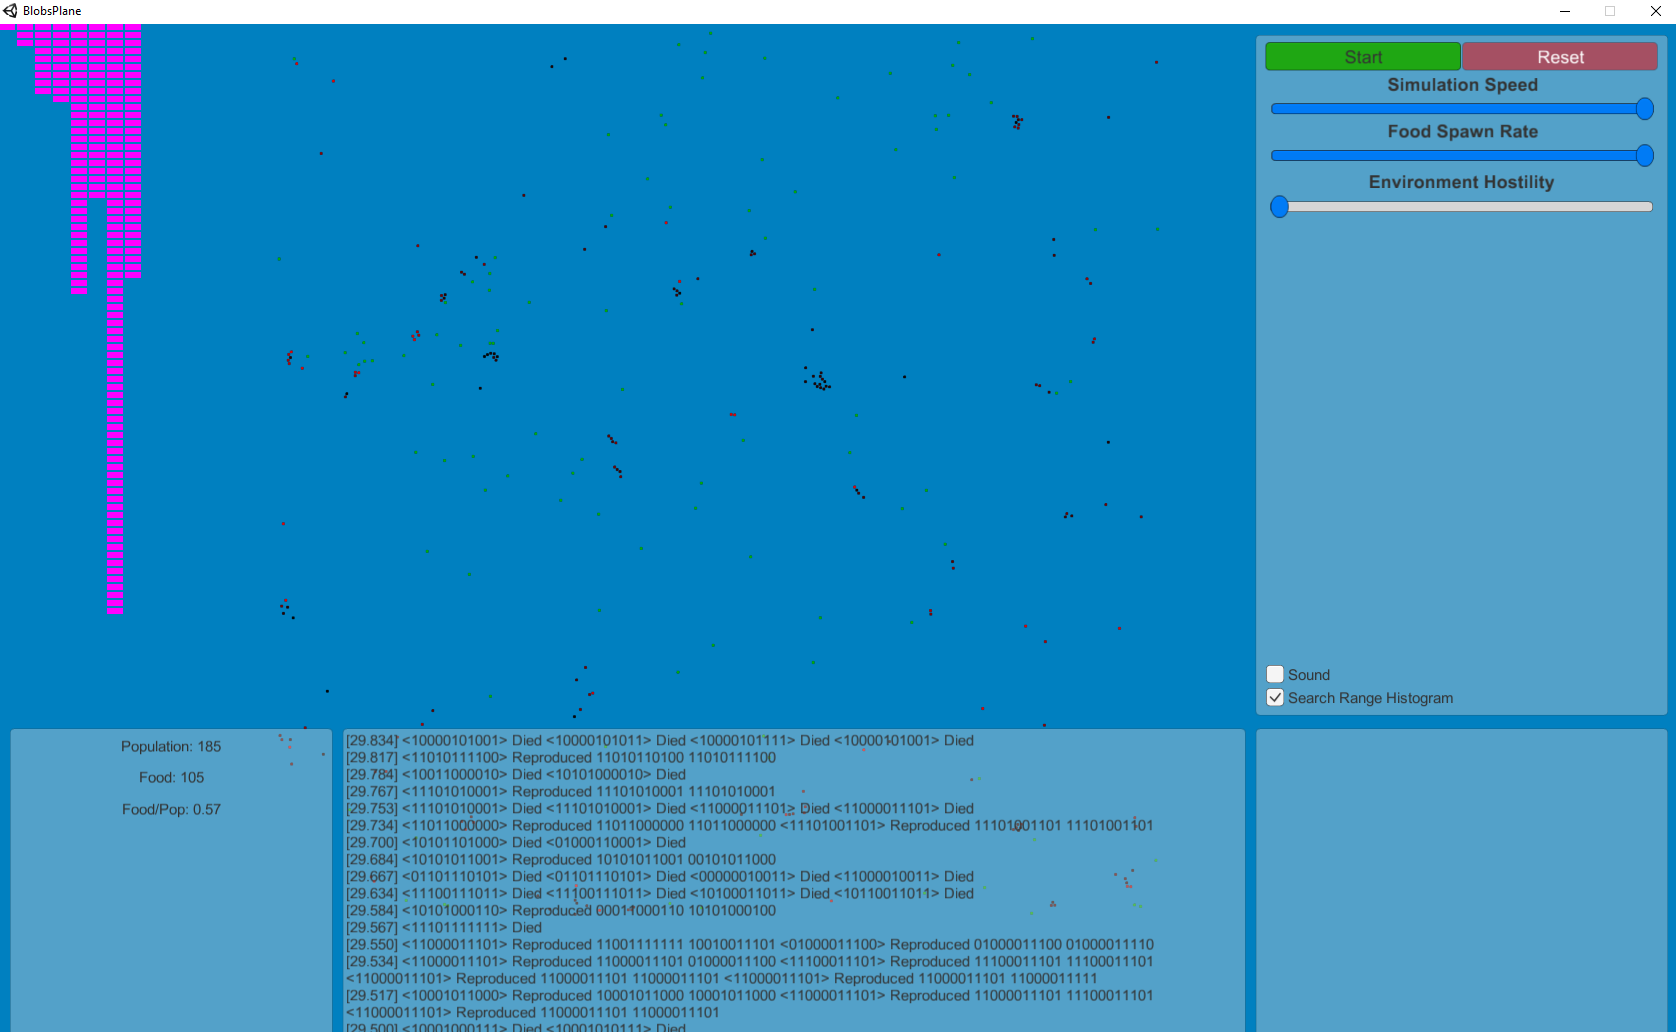
\includegraphics[scale=0.3]{images/unitypart}
	\caption{\label{fig:unitypart}One of the intermediary designs}
\end{figure}

Together with the line graph and the blob selection tool-tip, implantation of the camera changes led to the finalised design, as seen in Figure~\ref{fig:finalui}

\begin{figure}[!th]
	\centering
	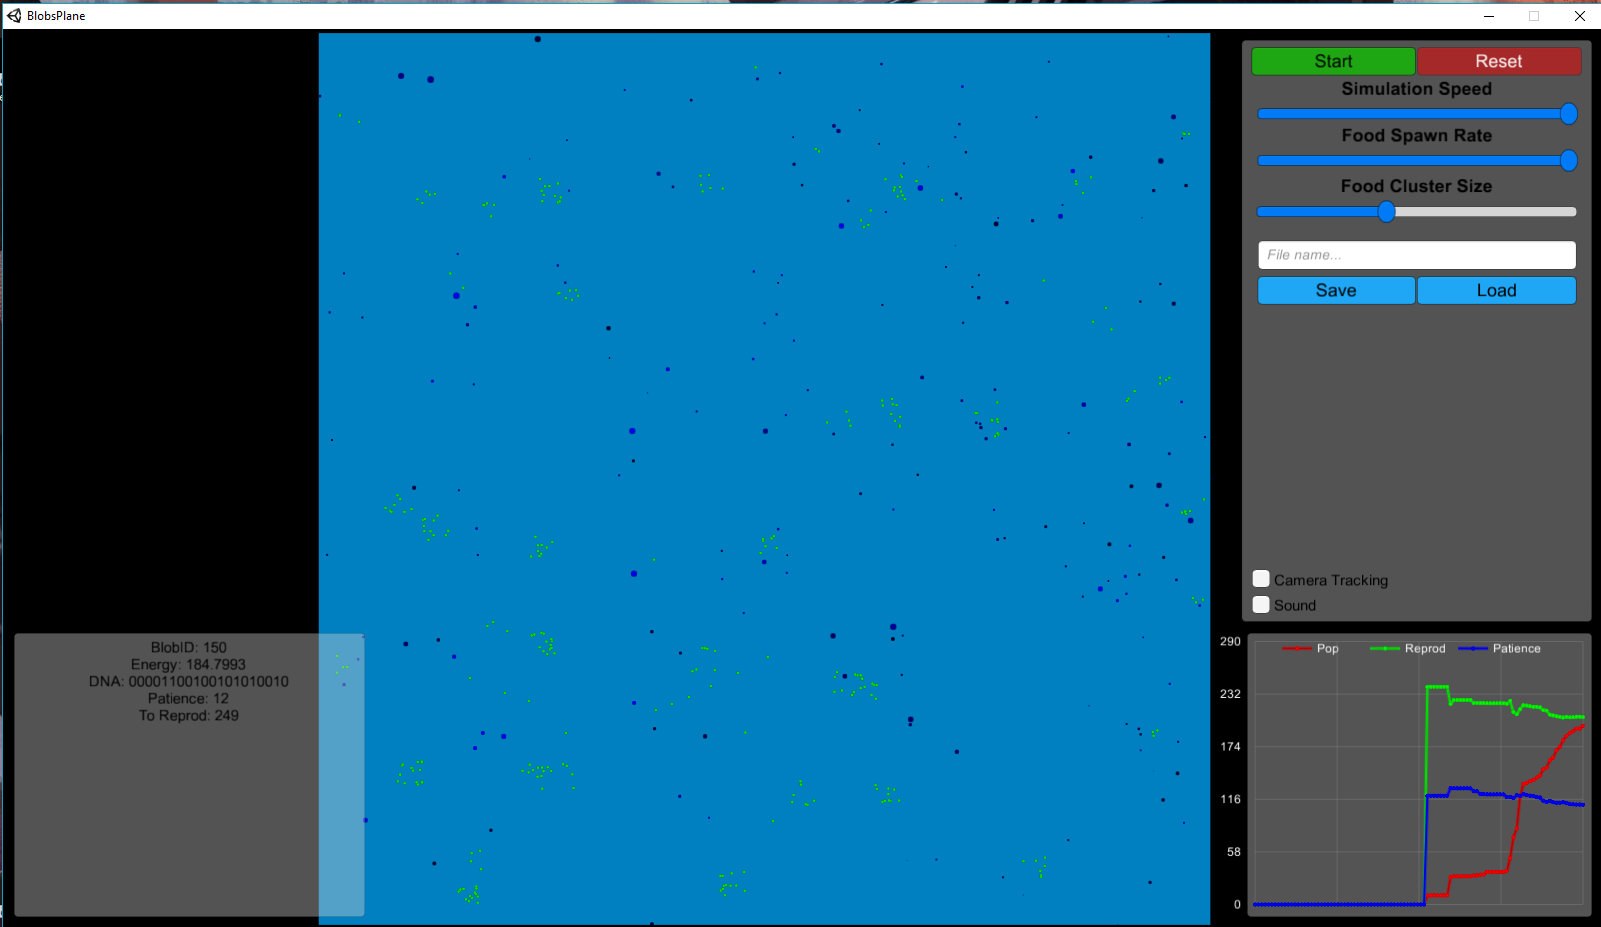
\includegraphics[scale=0.315]{images/finalui}
	\caption{\label{fig:finalui}Final design of the application}
\end{figure}

\subsection{Statistical Graph} \label{sgraph}

In the bottom-right of the application, a graph displaying information about the current population can be seen. An example is presented in Figure~\ref{fig:graph}. The data series available are: number of individuals, the average reproduction threshold amongst the population, and the average time until a blob leaves an area in search of food. Albeit few, these three parameters accurately represent trends within the population following significant environmental events, such as those described in Section~\ref{experiments}. The graph is created with the help of a library available through the Unity Asset Store as a purchasable Asset\cite{graphmaker}.

\begin{figure}[!th]
	\centering
	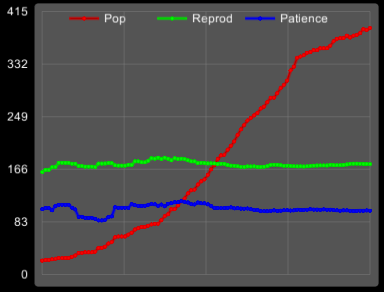
\includegraphics[scale=0.85]{images/graph}
	\caption{\label{fig:graph}A screenshot of the line graph}
\end{figure}

\section{Evolution Logic}

In the presence of food, blobs will just float in the general area. Once food levels decrease, the blobs simulate a type of random walk, named L\'evy walk. This is also used by bacteria, and is thought to be an optimal strategy for searching sparsely populated random environments\cite{viswanathan1999optimizing}, such as food distributed on a plane. To note is that the number of food pellets available cannot exceed a predefined maximum, in order to keep the population within manageable levels.

As the blobs gain energy by eating, they become visually larger, until they reach their reproduction threshold. This causes a blob to begin asexual reproduction, effectively splitting into two children. Energy is lost over time; should at any point a blob's energy reach zero, it would immediately die. A blob can be formally described as a finite-state machine, as seen in Figure~\ref{fig:fsm}.

\begin{figure}[!th]
	\centering
	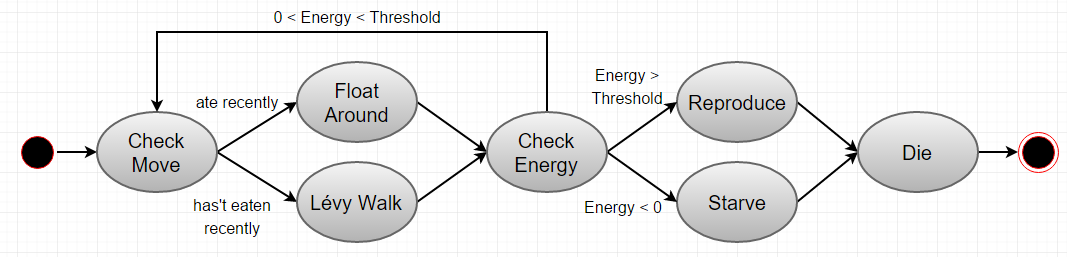
\includegraphics[scale=0.65]{images/fsm}
	\caption{\label{fig:fsm}A finite-state machine detailing a blob's behaviour}
\end{figure}

\subsection{Reproduction and DNA}
Reproduction was chosen to be asexual in order to simplify a blob's behaviour to its basics. Sexual reproduction would involve either the need to search for a partner, or the inherent randomness of blobs colliding and exchanging genes. This would add an unnecessary layer of complexity to the simulation. As such, a blob simply divides into two children in a manner similar to cytokinesis\cite{rappaport2005cytokinesis}.
Each child carries the DNA of its parent, with a slight variation dependant on whether a mutation occurred. Encoded in a blob's DNA are its two main characteristics: the reproduction threshold and the time needed until it starts searching for a new food source.